\section{Interface - Contexts}

\begin{frame}

\frametitle{Princip}

\underline{Old cryptographic interface (Crypto Wrap)}:
\begin{itemize}
  \item Several functions with only one parameter of difference
  \item Several times the same parameters added for doing the same thing
\end{itemize}

\vspace{0.25cm}

\underline{New cryptographic interface (GCI)}:
\begin{itemize}
  \item Use of context to save one time the parameters
  \item Give an identifiant (ID) back with where are the parameters saved
  \item Use of the ID to update the datas and get the result
  \item Release the context (the parameters in the same time) to free memory
\end{itemize}

\end{frame}


\begin{frame}

\frametitle{Example of use:}


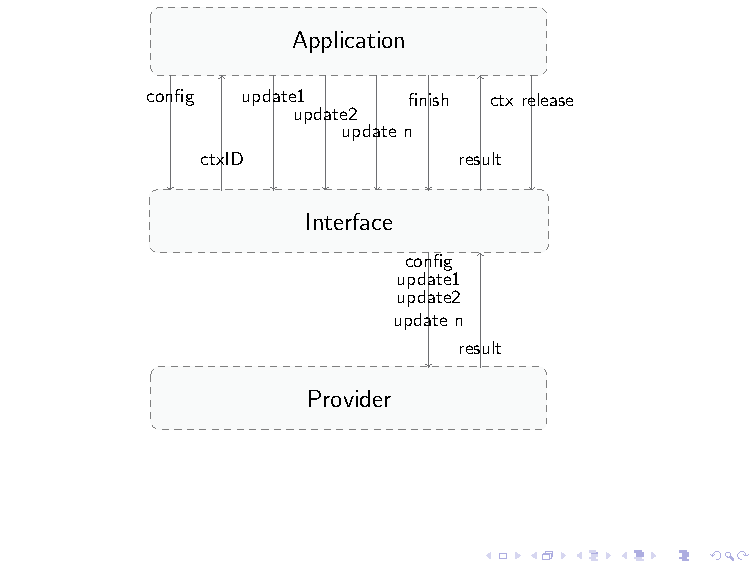
\includegraphics[trim=0.5cm 1cm 14cm 0cm, height=8cm]{figures/context.pdf}


\end{frame}
